\documentclass{article}
\usepackage[utf8]{inputenc}
%Pacchetto per le equazioni matematiche
\usepackage{amsmath}
%Pacchetto per i grafici
\usepackage{graphicx}

\title{Progetto Controlli 3A}
\author{
    Luca Bartolomei 
    \texttt{0000825005}
    \\
    Federico Maria Macchiavelli 
    \texttt{0000825621}
    \\
    Mattia Innocenti 
    \texttt{0000825046}
    \\
    Andrea Proia 
    \texttt{0000825784}
}

\date{Dicembre 2019}

\begin{document}

\maketitle

\section{Introduzione}

Progettazione di un controllore per un impianto idroelettrico, mediante l'utilizzo delle tecniche di controllo.

\section{Impianto idroelettrico}

L'impianto idroelettrico è modellato come sistema SISO avente due variabili di stato (la pressione  dell’acqua sul fondo del bacino ($x_1$) e la portata in uscita dal bacino ($x_2$ )). Le equazioni differenziali che modellano le variabili di stato sono di tipo non lineare:

$$
\begin{array}{lcl}
    \dot{x}_1 & = & 0 \\
    \dot{x}_2 & = & -C_d u x_2 |x_2| -R_0 x_2 |x_2| + x_1
\end{array}
$$

L'uscita del sistema viene modellata secondo la formula,:

$$
\begin{array}{lcl}
    y & = & -\eta x_1 x_2
\end{array}
$$

Anche la $y$ è di tipo non lineare.

\subsection{Significato fisico}

Il sistema modella la pressione sul fondo del bacino come costante, mentre la variazione nel tempo della portata nel fondo del bacino dipende da tre fattori:

\begin{itemize}
    \item Pressione sul fondo del bacino $x_1$: Una pressione positiva contribuisce ad aumentare la portata nel fondo del bacino
    \item Perdite di carico nella condotta $-R_0 x_2 |x_2|$: Si tratta dell'attrito tra la condotta e l'acqua, che contribuisce a diminuire la portata
    \item Valvola di controllo $-C_d u x_2 |x_2|$: Consiste in una valvola che se opportunamente controllata permette di aumentare l'effetto di perdita di carico nella condotta. L'effetto della valvola è condizionata dalla portata attuale.
\end{itemize}

L'uscita $y=-\eta x_1 x_2$ rappresenta la potenza elettrica generata dall'impianto. Viene calcolata come la potenza fluidica $x_1 x_2$ e moltiplicata per un coefficiente che indica l'efficienza di conversione tra energia meccanica e energia elettrica. Il segno negativo è dovuto al trasduttore utilizzato: per esempio se generiamo 1MW di potenza, avremmo in lettura dal sensore -1MW. Aprendo o chiudendo la valvola possiamo cambiare la potenza in uscita.

%TODO: nota sul gradino negativo necessario per la logica negativa del sistema

\subsection{Progettazione fisica del controllo}

Ragionando in termini di progettazione reale, il segnale ricevuto dal trasduttore di potenza sarà di tipo elettrico, il quale verrà elaborato da un circuito elettronico analogico/digitale, realizzato secondo la rete regolatrice da noi progettata. 
Infine anche il segnale di controllo sarà di natura elettrica, quindi necessitiamo di un attuatore, per esempio un motore elettrico o un solenoide, magari con circuiteria aggiuntiva di potenza e di un sistema meccanico per l'interfacciamento valvola-motore, per controllare la valvola, oppure si potrebbe sostituire la valvola con una elettro-valvola, avente attuatore già incluso.

\section{Specifiche}

L'azienda che ci ha assunto ha fornito delle specifiche sul sistema di controllo andremmo a progettare:

\begin{itemize}
    \item Errore a regime nullo ($e_{\infty}=0$) per un gradino di ampiezza 30
    \item Sovraelongazione percentuale minore del 5\%
    \item Tempo di assestamento all'1\% minore di 0.3 sec
    \item Attenuazione dei rumori di misura di almeno 30 volte (a partire da una pulsazione $\omega_n=1000 rad/s$)
    \item Margine di fase di almeno 45 gradi
\end{itemize}

Si aggiungono delle opzioni facoltative:
\begin{itemize}
    \item Aumento delle performance del sistema di controllo, modificando il tempo di assestamento all'1\% il quale dovrà essere minore di 0.033 sec
    \item Analisi delle performance del regolatore sul sistema non lineare in un intorno della coppia di equilibrio.
\end{itemize}

\section{Linearizzazione del sistema}

Per prima cosa linearizziamo il sistema idroelettrico in un sistema lineare. Per fare ciò utilizziamo la coppia di equilibrio fornita $x=(10,6), u=(\frac{\frac{x_1}{x_2 |x_2|}-R_0}{C_d})$:

Mediante la linearizzazione troviamo le quattro matrici $A,B,C,D$:

$$
A=
\begin{bmatrix}
    0 & 0\\
    1 & -3.333
\end{bmatrix}
B=
\begin{bmatrix}
    0\\
    -710.6115
\end{bmatrix}\\
C=
\begin{bmatrix}
    -3.6 & -6
\end{bmatrix}
D=0
$$

Da esse si ricava la funzione di trasferimento:

$$
G=\frac{4263.7 s}{s (s+3.333)}
$$

\subsection{Verifica delle prestazioni ad anello chiuso}

Analizziamo la rispsta al gradino del sistema senza regolatore in retroazione:

\begin{center}
    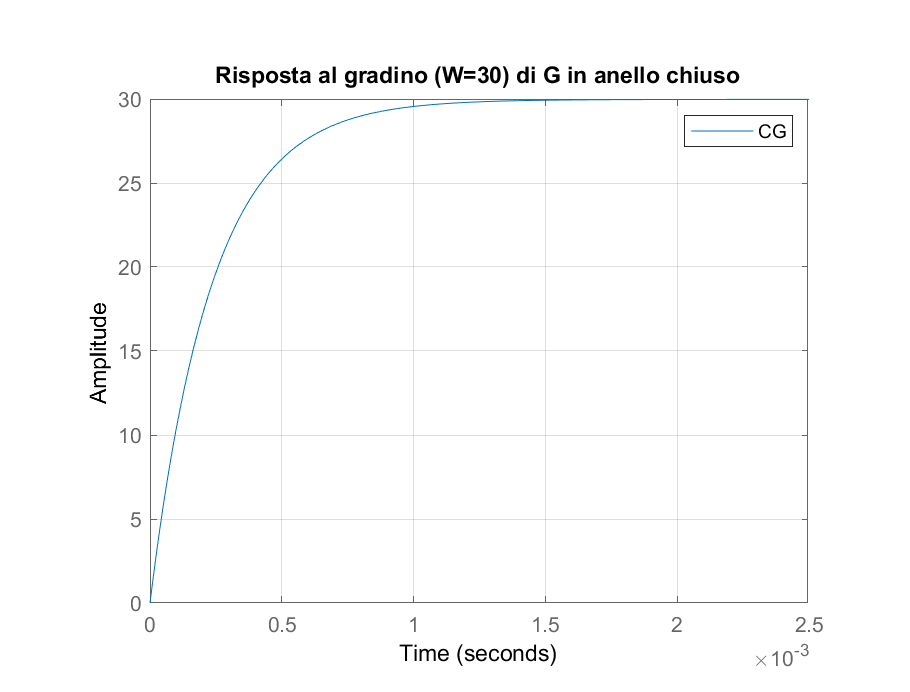
\includegraphics[scale=0.6]{figure1.eps}
\end{center}

Dalla figura possiamo evidenziare le sequenti performance:

\begin{itemize}
    \item Tempo di assestamento all'1\% molto basso, minore di 0.01 sec
    \item Sovraelongazione percentuale inferiore al 5\%
\end{itemize}

Il sistema però non soddisfa alcune caratteristiche richeste:

\begin{itemize}
    \item Errore a regime non nullo (ma comunque basso visto l'alto guadagno del sistema in anello aperto)
    \item Attenuazione del rumore di misura quasi nullo
\end{itemize}

In conclusione abbiamo bisogno di un regolatore per risolvere le problematiche del sistema in retroazione.

\section{Progettazione del regolatore}

\subsection{Progettazione della rete regolatrice statica}

Per garantire un errore a regime nullo abbiamo bisogno di un regolatore statico:

$$
R_s(s)=\frac{1}{s}
$$

Il guadagno $\mu_s$ risulta libero e può essere usato successivamente se ci ritroveremo in uno scenario A.

Proviamo a disegnare il diagramma di Bode per verificare in quale scenario ci siamo collocati.

\begin{center}
    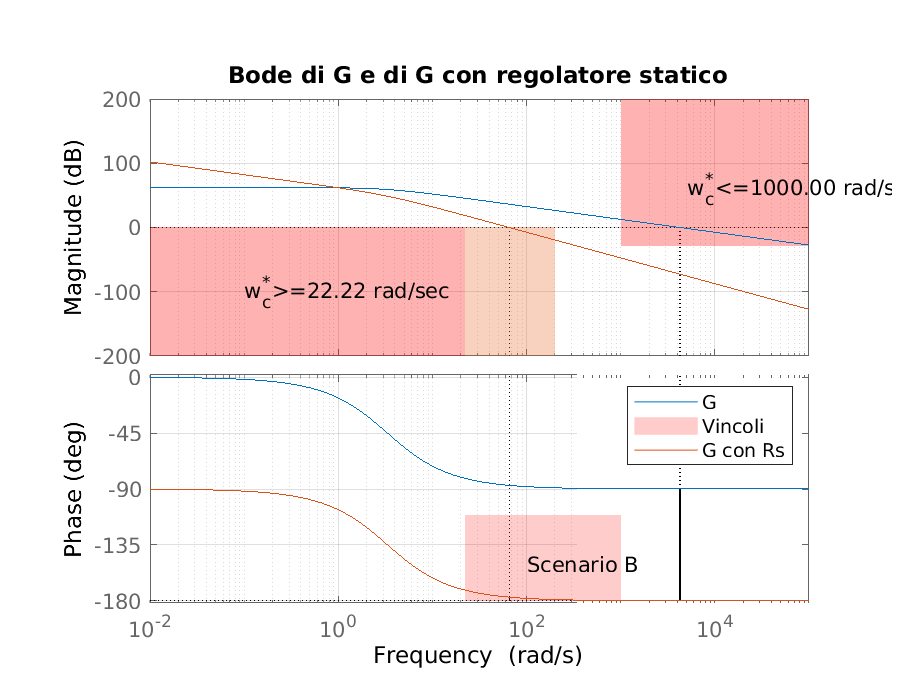
\includegraphics[scale=0.8]{figure2.eps}
\end{center}

Osservando il diagramma di Bode della fase deduciamo che siamo caduti in uno scenario di tipo B, in quanto non esiste un range di pulsazioni $\omega$ in cui $G_e(j\omega)$ rispetta il vincolo sul margine di fase.

\subsection{Progettazione della rete regolatrice dinamica}

Per ovviare allo scenario B, abbiamo bisogno di un regolatore dinamico formato da una rete anticipatrice.

$$
R_d(s)=\frac{1+\tau s}{1+\tau \alpha s}
$$

Il polo presente della rete anticipatrice è dovuto alla fisica realizzabilità della rete.

Rimane il problema di dove porre lo zero e il polo nel piano complesso:
\begin{itemize}
    \item Lo zero deve fornire un aumento di fase tale da superare il vincolo del margine di fase in almeno una parte del range di attraversamento
    \item Il polo deve essere collocato in alta frequenza (lontano dall'asse degli immaginari) per non disturbare l'effetto dello zero.
\end{itemize}

Invece che utilizzare le formule di inversione, abbiamo preferito progettare la rete per \textbf{cancellazione}: in questo modo riusciamo a ricondurre il sistema ad uno equivalente del primo ordine, a meno di una coda di assestamento dovuta ad una incertezza di posizionamento dello zero rispetto al polo del sistema in -3.333:

$$
\begin{array}{lll}
    R_d(s) = \frac{(s+3.333)}{(s+333.3)} &\alpha=0.01 & \tau=\frac{1}{3.333}
\end{array}
$$

Tecnicamente il polo della rete anticipatrice non dovrebbe superare la pulsazione di attraversamento, altrimenti non potremmo disegnare il vincolo di attraversamento minimo nel diagramma di Bode, in quanto la pulsazione di attraversamento non corrisponderebbe e la condizione $\omega_n\approx\omega_c$ non sarà valida.\\

Utilizzando il luogo delle radici per imporre il vincolo di attraversamento minimo, il quale non è altro che la specifica di tempo di assestamento, unito al fatto che durante i test abbiamo constatato che la pulsazione di attraversamento non varia di molto, possiamo trascurare questo vincolo.

\subsection{Calcolo di $\mu_d$ per il rispetto dei vincoli}

Per calcolare i vincoli di sovraelongazione e di tempo di assestamento abbiamo utilizzato il luogo delle radici, dato che il guadagno statico era libero. Mentre per calcolare il guadagno statico neccessario per il vincolo sull'attenuazione dei rumori di misura abbiamo utilizzato il diagramma di Bode.

\subsubsection{Attenuazione necessaria per il rumore di misura}

Utilizzando le funzioni di Matlab e il diagramma di Bode, abbiamo calcolato il valore massimo di $\mu_d$, ancora libero in quanto non usato nel regolatore statico, per rispettare il vincolo di attenuazione di misura.

$$
    \mu_{d_B}=0.0734
$$

\newpage

\subsubsection{Vincolo di $\mu_d$ per la specifica di sovraelongazione}

Utilizzando il luogo delle radici siamo riusciti a calcolare il valore \textbf{massimo} di $\mu_d$ per rispettare il vincolo di sovraelongazione.

\begin{center}
    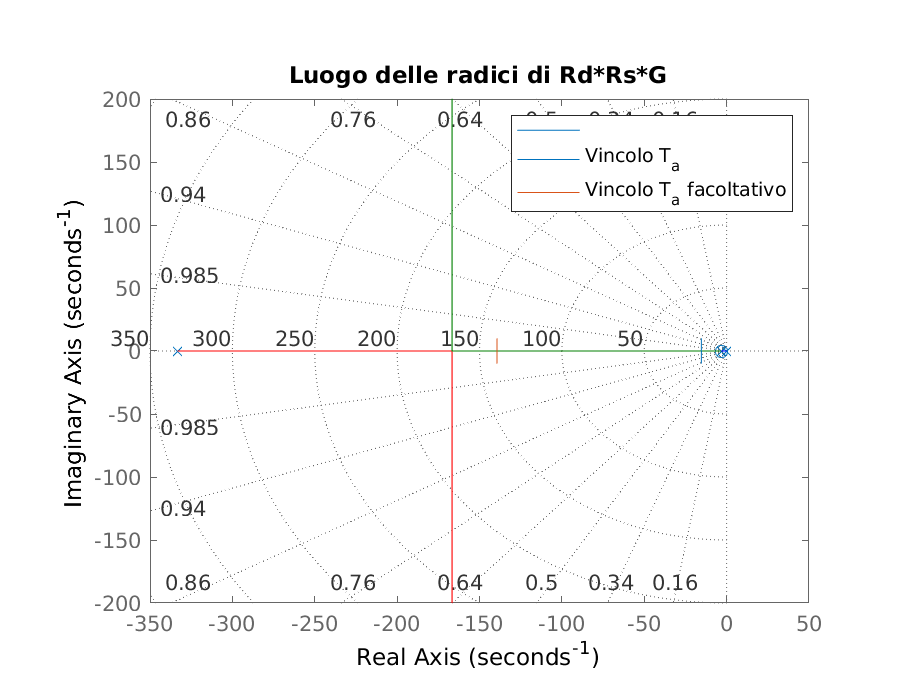
\includegraphics[scale=0.7]{figure4.eps}
\end{center}
Infatti andando in retroazione si vengono a creare due poli complessi coniugati che possono violare i vincoli di sovraelongazione.\\
Tenendo il guadagno sotto una soglia massima data da $\xi=0.69$, perfettamente visibile utilizzando il \texttt{grid on} abbiamo riscontrato un $\mu_d$:

$$
    \mu_{d_S} = 0.106
$$

Che risulta meno stringente rispetto al vincolo $\mu_{d_B}$.

\subsubsection{Vincolo di $\mu_d$ per il tempo di assestamento}

Un ultimo vincolo del guadagno è dato dal tempo di assestamento, il quale si traduce in un asse parallelo all'asse degli immaginari. Ciò comporta un valore \textbf{minimo} che il guadagno deve rispettare.\\

Sempre dalla figura del luogo delle radici, dopo aver disegnato gli assi del tempo di assestamento, si ricava un vincolo per $\mu_d$:

$$
    \mu_{d_T} = 0.0498
$$

\newpage

\subsubsection{Selezione di $\mu_d$}

In conclusione abbiamo preso un guadagno $\mu_d$ tale che rispetti i vincoli $\mu_{d_B}$, $\mu_{d_S}$, $\mu_{d_T}$:

$$
\begin{cases}
    \mu_{d_B}\geq\mu_d\\
    \mu_{d_S}\geq\mu_d\\
    \mu_{d_T}\leq\mu_d
\end{cases}
$$

Abbiamo scelto $\mu_{d_B}$ come guadagno, in quanto rispetta i vincoli.


\begin{center}
    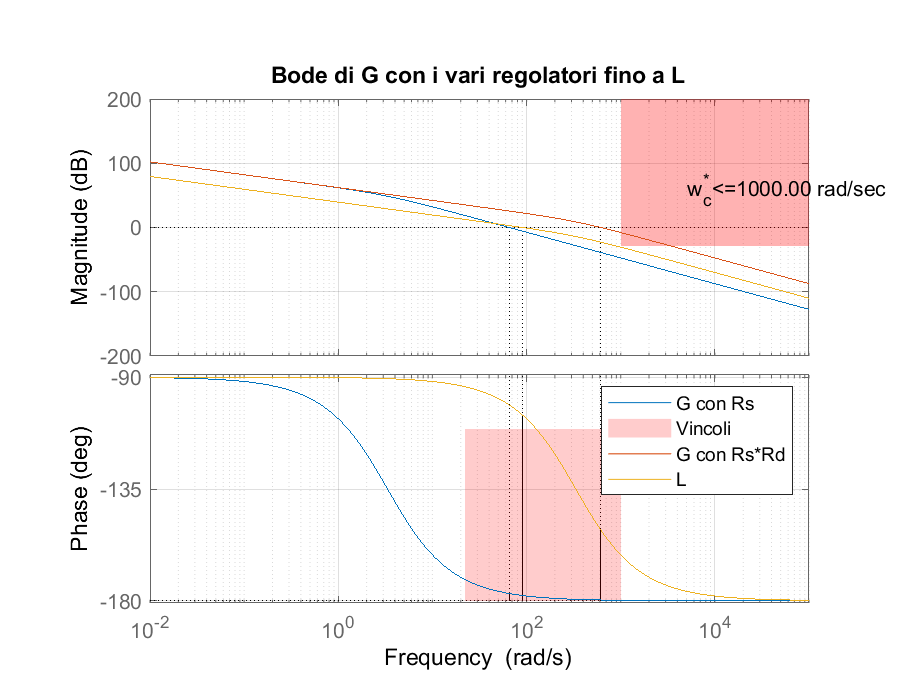
\includegraphics[scale=0.8]{figure3.eps}
\end{center}

Dal diagramma di bode si può notare il rispetto del vincolo di attenuazione di misura e il rispetto del margine di fase, già visto nel luogo delle radici.

\section{Funzione ad anello aperto e di sensitività}

$$
\begin{array}{cc}
    L_{+20\%}(s)=\frac{31315 s (s+4)}{s^2 (s+333.3) (s+3.333)} & F_{+20\%}(s)=\frac{31315 s^3 (s+333.3) (s+4) (s+3.333)}{s^3 (s+333.3) (s+4.029) (s+3.333) (s^2 + 332.6s + 31090)}
\end{array}
$$

Possiamo approssimare $F(s)$ ad un sistema del secondo ordine con poli complessi coniugati dominanti per effetto delle cancellazioni. La quasi cancellazione porterà una coda di assestamento, che potrebbe influire negativamente.


\newpage

\section{Verifica delle performance}

\subsection{Verifica delle performance sul sistema linearizzato}

Una volta ottenuto la funzione ad anello aperto, abbiamo imposto la retroazione:
$$
F = \frac{L}{1+L}
$$

\subsubsection{Verifica di $e_\infty=0$, $S\%$, $T_{a_0}$, $M_f$}

\begin{center}
    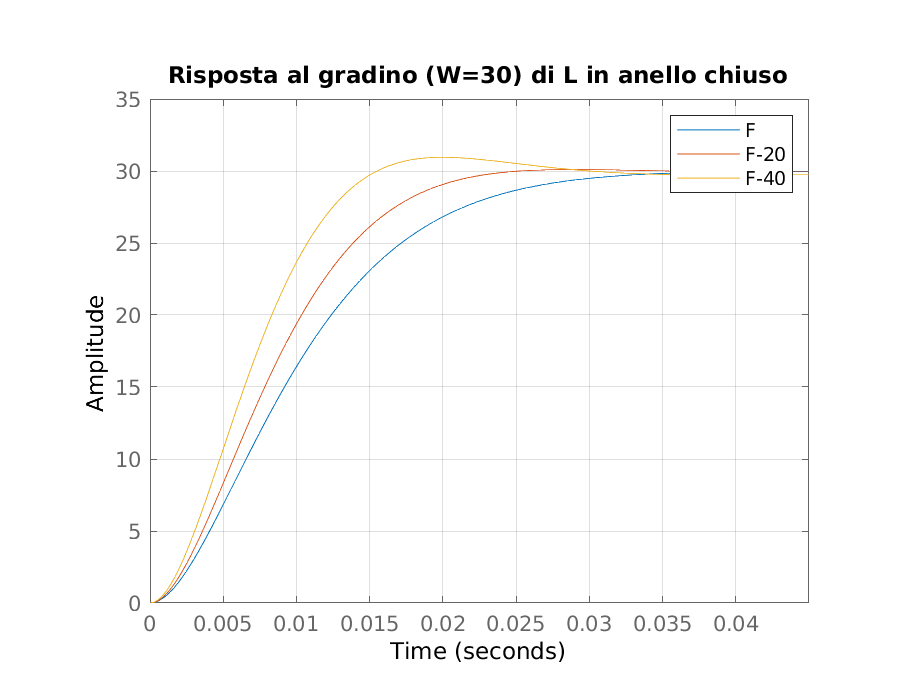
\includegraphics[scale=0.7]{figure5.eps}
\end{center}

Si può notare l'aggiunta delle risposte al gradino con le incertezze sulla rete anticipatrice fino al 20\%. L'aumento della sovraelongazione per F$\pm20\%$ è dovuta allo spostamento dello zero. Si ricorda che l'incertezza sullo zero induce una \textbf{correzione sul guadagno}.\\

Abbiamo testato la rete mediante \texttt{stepinfo}, impostando il gradino avente ampiezza $W$, mediante comando \texttt{StepAmplitude} e rilevazione del tempo di assestamento all'1\% mediante comando \texttt{SettlingTimeThreshold}:

\begin{itemize}
    \item \textbf{SettlingTime}: 0.0321 sec
    \item \textbf{Overshoot}: 0 \%
\end{itemize}

Di conseguenza le specifiche di tempo di assestamento, margine di fase e di sovraelongazione sono rispettate. Guardando il grafico di step, la specifica $e_\infty=0$ sembra rispettata. 

\subsubsection{Verifica attenuazione disturbo di misura ($B_n$)}

La verifica sull'attenuazione dei rumori di misura viene effettuata mediante diagramma di Bode.

\begin{center}
    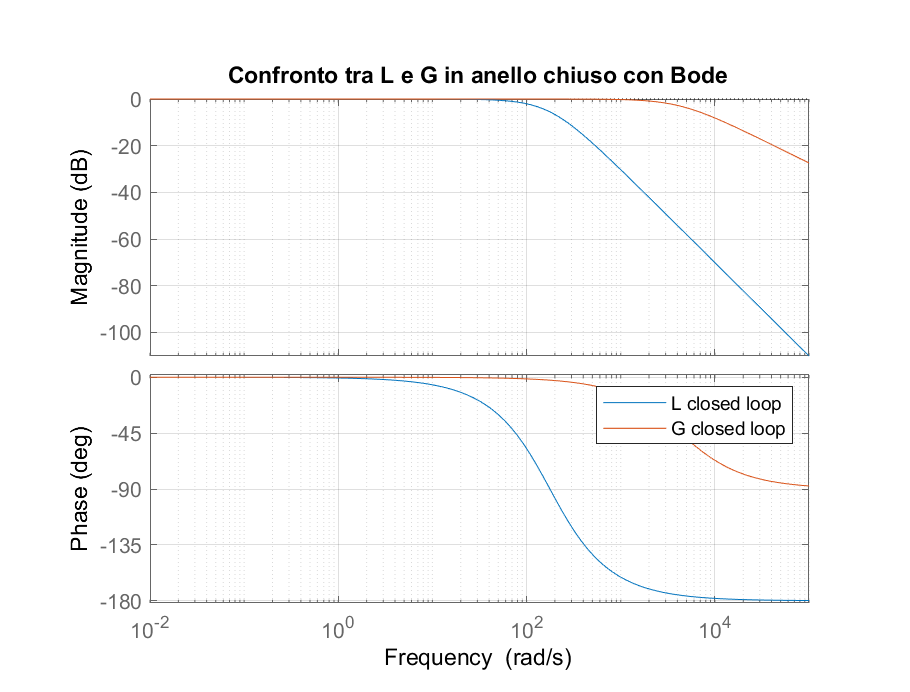
\includegraphics[scale=0.9]{figure6.eps}
\end{center}

Si può notare che alla pulsazione $\omega_n=1000 rad/s$ abbiamo un'attenuazione di -30db, soddisfando la specifica.\\\\

Si può vedere che la specifica viene rispettata andando a simulare il sistema tramite Simulink, con in quale è possibile introdurre un errore di misura (\texttt{sineWave}).

\subsubsection{Conclusioni sull'analisi}

Il regolatore progettato rispetta tutte le specifiche richieste, almeno per quanto riguarda il sistema linearizzato.

\newpage

\subsection{Verifica delle performance con il sistema non lineare}
Abbiamo effettuato delle verifiche sulle performance del regolatore sul sistema non lineare. Abbiamo testato un ingresso a gradino con ampiezza $W$ e un altra simulazione con ampiezza $-W$.

\subsubsection{Performance con $W$}

\begin{center}
    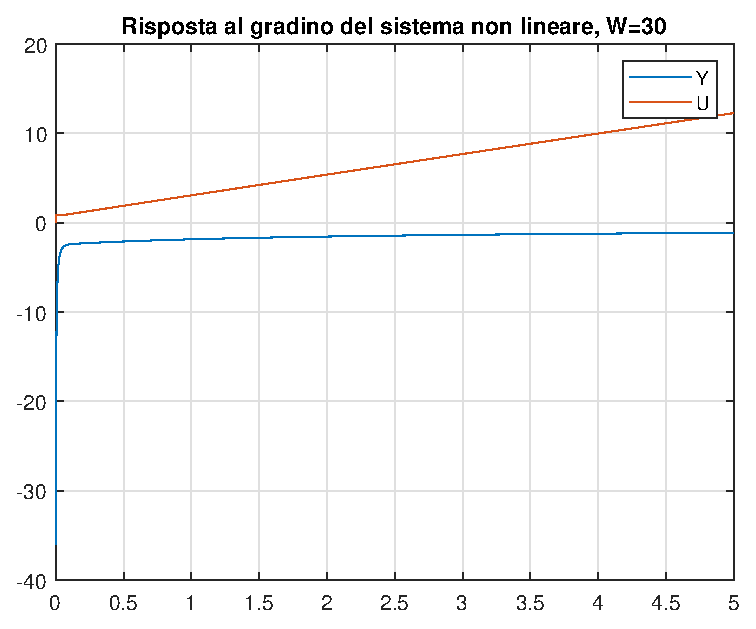
\includegraphics[scale=0.9]{figure8.eps}
\end{center}

Dal grafico si nota che il regolatore \textbf{non funziona} a dovere. Ciò è dovuto al sensore a logica \textbf{negativa} e alla natura non lineare del sistema: il prodotto $-C_d u x_2 |x_2|$ presente in $\dot{x_2}$ crea una \textbf{dipendenza} tra $u$ e $x_2$. Nel sistema lineare invece il prodotto precedente viene \textbf{sostituito da una somma}, \textbf{rimuovendo la dipenzenza tra i due}.\\\\
Cosi facendo il sistema linearizzato ammette gradini positivi, mentre il sistema non lineare, sotto le condizioni iniziali, \textbf{non li ammette}. Potremmo interpretare fisicamente il fenomeno come un comando di \textbf{assorbire} energia, invece che produrla, invertendo la portata, dato che la pressione è costante.

\newpage

\subsubsection{Performance con $-W$}

Se ripetiamo il test con $-W$, dopo un breve transitorio, non previsto nel sistema linearizzato, l'uscita si assesta sul valore desiderato:

\begin{center}
    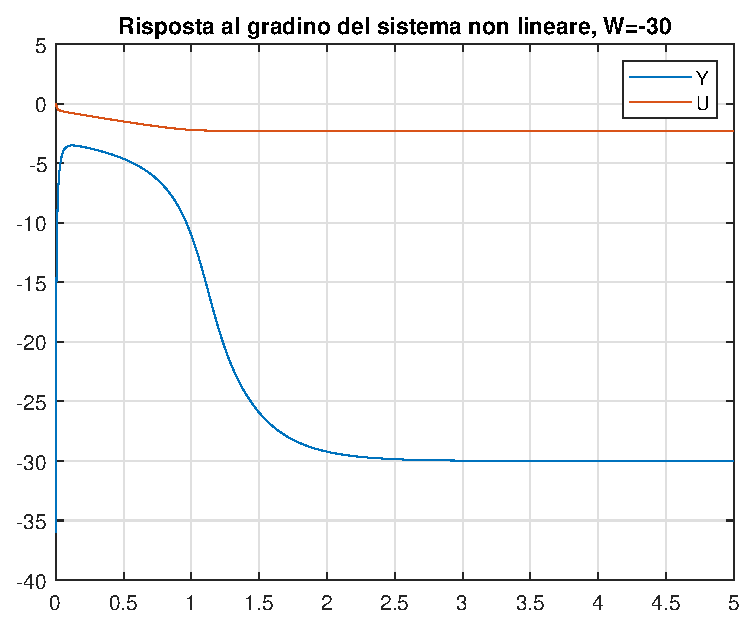
\includegraphics[scale=0.8]{figure9.eps}
\end{center}

Il risultato va preso con le pinze, in quanto abbiamo che la valvola, invece che aumentare le perdite di carico, le \textbf{riduce}.

\subsubsection{Nota sulla fisica realizzabilità}
Se volessimo che la valvola aumenti soltanto le perdite, dovremmo imporre $1\geq u \geq0$ e forti vincoli sulla potenza massima generata dal sistema ($W$), come ci aspetteremmo da un impianto idroelettrico reale.

\section{Conclusioni}

Il sistema linearizzato è stato correttamente regolato in base alle specifiche date, tenendo in conto anche della specifica facoltativa $T_{a_0}$. Inoltre abbiamo analizzato il sistema mediante gradino. L'incertezza sullo zero della rete anticipatrice induce una correzione del guadagno a \textit{run-time}.\\

Il sistema non lineare si comporta differentemente, a seconda del segno dell'ampiezza del gradino all'ingresso. Ciò è causato dalla logica negativa del sensore e da effetti non lineari, non presenti nel sistema linearizzato.

\end{document}

